\documentclass[12pt]{article}
\usepackage[utf8]{inputenc}
\usepackage[T2A]{fontenc}
\usepackage[english, russian]{babel}
\usepackage{array}
\usepackage{makecell}
\usepackage{enumitem}
\usepackage{graphicx}%Вставка картинок правильная

\usepackage{float}%"Плавающие" картинки

\usepackage{wrapfig}%Обтекание фигур (таблиц, картинок и прочего)
\graphicspath{{noiseimages/}}
\usepackage{amsmath, amsfonts, amssymb, amsthm}
\usepackage{fancybox, fancyhdr}
\usepackage{multicol}
\usepackage{multirow}
\usepackage[left = 1cm, right = 2cm, top = 2cm, bottom = 2cm, bindingoffset = 1cm]{geometry}
\newcommand\tab[1][1,15cm]{\hspace*{#1}}
\newcommand{\specialcell}[2][c]{%
  \begin{tabular}[#1]{@{}c@{}}#2\end{tabular}}
    
\begin{document}
    
    \begin{figure}[H]
    
        \centering
        
        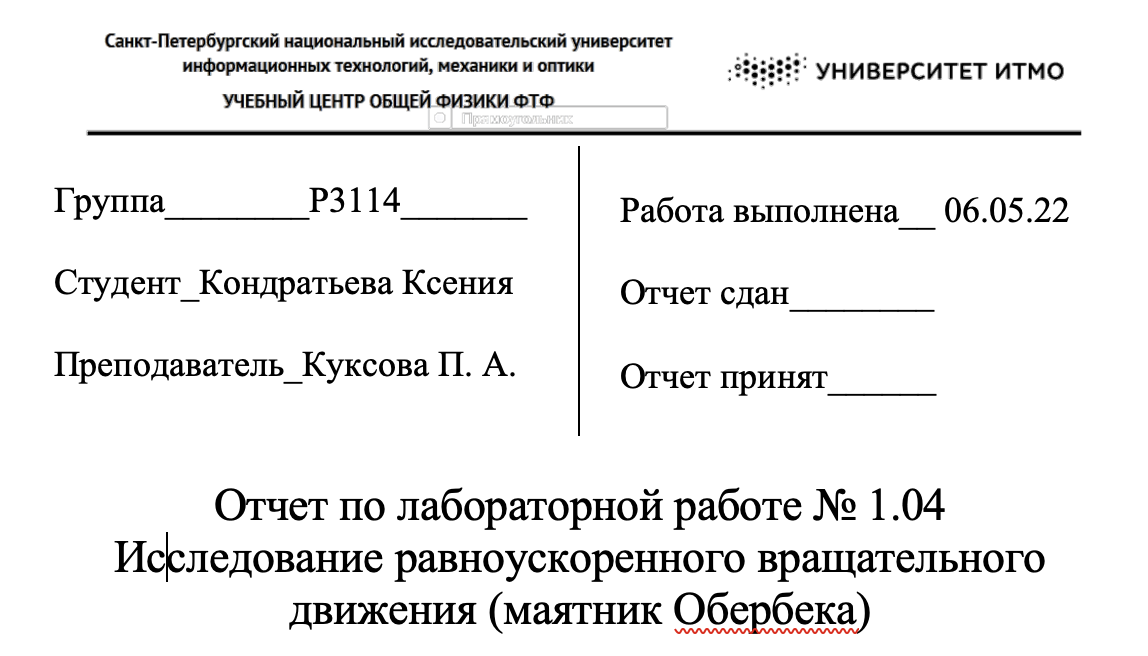
\includegraphics[width=1.05\linewidth]{title.png}
        \label{fig:mpr}
        
    \end{figure}

    
    \begin{enumerate}[label=\arabic*)]
        \item Цель работы.
            \begin{itemize}
                \item Проверка основного закона динамики вращения.
                \item Проверка зависимости момента инерции от положения масс относительно оси вращения.
            \end{itemize}
        
        \item Задачи, решаемые при выполнении работы.
            \begin{itemize}
                \item Измерение времени падения грузов с различными массами, которые раскручивают вращательный маятник.
                
                \item Вычисление значений исследуемых величин по приведенным формулам
            
                 \item Построение графиков зависимости по результатам измерений
            \end{itemize}
        
        \item Объект исследования.
            \begin{itemize}
                \item  Падающий груз и маятник Обербека.
            \end{itemize}
          
        
        
        \item Метод экспериментального исследования.
            \begin{itemize}
                \item  Многократные измерения.
            \end{itemize}
        
        \item Рабочие формулы и исходные данные.
        \begin{itemize}
                \item Второй закон Ньютона:
                \begin{gather} 
                ma = mg - T 
                \end{gather}
                
            
                \item Ускорение a:
                \begin{gather} 
                a = \frac{2h}{t^2}
                \end{gather}
                
                \item Угловое ускорение $\varepsilon$, где $d$ - диаметр ступицы:
                \begin{gather} 
                \varepsilon = \frac{2a}{d}
                \end{gather}
                
                \item Момент силы натяжения нити:
                \begin{gather} 
                M = \frac{md}{2}(g-a)
                \end{gather}
                
                \item Основной закон динамики вращения для крестовины:
                \begin{gather} 
                    I\varepsilon = M - M_{\text{тр}}
                \end{gather}
                
                \item Момент инерции крестовины с грузом:
                \begin{gather} 
                    I = I_0+4m_{\text{ут}}R^2
                \end{gather}
                
                \item Расстояние между осью O вращения и центром грузика:
                \begin{gather} 
                    R = l_1 - (n-1)l_0+ \frac{1}{2}b
                \end{gather}
                
                \item Значение момента инерции крестовины для каждого положения грузов:
                \begin{gather} 
                    I = \frac{\sum_{i=1}^3(\varepsilon_i-\varepsilon_{\text{ср}})(M_i-M_{\text{ср}})}{(\varepsilon_i-\varepsilon_{\text{ср}})^2}
                \end{gather}
                
                \item Значение момента силы трения для каждого положения грузов:
                \begin{gather} 
                    M_{\text{тр}} = M - I\varepsilon
                \end{gather}
            
                
                \item Абсолютная погрешность прямых измерений:
                \begin{gather} 
                    \Delta x' = \sqrt{\Delta x_{\text{ср}}^2 + \Big(\frac{2}{3} \Delta_{\text{их}}\Big)^2}
                \end{gather}
                
                \item Относительная погрешность прямых измерений:
                \begin{gather} 
                    \varepsilon_x = \frac{\Delta_x}{x_{\text{ср}}} * 100\%
                \end{gather}
                
                \item Абсолютная погрешность косвенных измерений:
                \begin{gather} 
                    \Delta_z = \sqrt{\Big(\frac{\delta z}{\delta a} \Delta_a\Big)^2 + \Big(\frac{\delta z}{\delta b}\Delta_b\Big)^2 ...}
                \end{gather}
                
                \item Относительная погрешность косвенных измерений:
                \begin{gather} 
                    \Delta\varepsilon_z = \frac{\Delta_z}{z_{\text{ср}}} * 100\%
                \end{gather}
                
                
                
                
        \end{itemize}
        
        
        \item Измерительные приборы.
        \begin{table}[H]
        \centering
                \begin{tabular}{|c|c|c|c|c|}
                \hline
                № п/п & Наименование & Тип прибора & Используемый диапазон & Погрешность\\
                \hline
                1 & Секундомер & Электронный & 0 - 8,70 с.& 0,05 с\\
                \hline
                2 & Линейка & Стационарный & 0 - 700 мм & 0,5 мм\\
                \hline
                \end{tabular}
        \end{table}
        
    
        \begin{figure}[H]
                \centering
                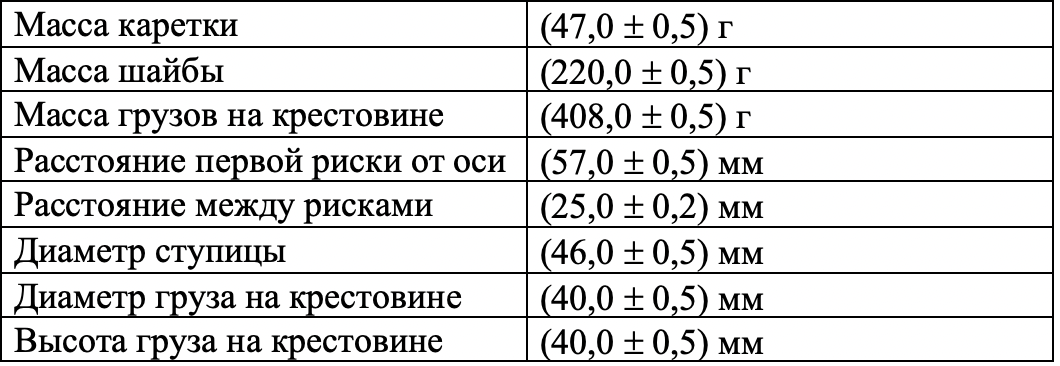
\includegraphics[width=0.75\linewidth]{3.png}
    
        \end{figure}
           
        
        
        \item Схема установки.
        
            \begin{figure}[H]
                \centering
                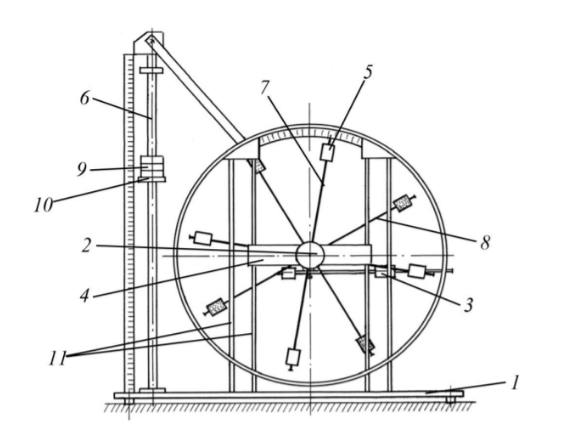
\includegraphics[width=0.75\linewidth]{system.png}
                \label{fig:mpr}
            \end{figure}
            \begin{center}
                 1 - основание, 2 - рукоятка сцепления крестовин, 3 - устройство принудительного трения, 4 - поперечина, 5 - груз крестовины, 6 - трубчатая направляющая, 7 - передняя крестовина, 8 - задняя крестовина, 9 - шайбы каретки, 10 - каретка, 11 - система передних стоек.
            \end{center}
        
        \item Результаты прямых измерений и их обработки.
        
        \begin{table}[H]
                \centering
                \begin{tabular}{|c|c|c|c|c|c|c|c|}
                    \hline
                    \multirow{2}*{Масса груз, кг} & \multirow{2}*{Время, с} & \multicolumn{6}{|c|}{Положение утяжелителей}\\
                    \cline{3-8}
                    & & 1 риска & 2 риска & 3 риска & 4 риска & 5 риска & 6 риска\\
                    \hline
                    \multirow{4}*{0,22} & t_1 & 4,58&	5,25&	5,91&	7,60&	8,62&	9,63\\
                    \cline{2-8}
                    & t_2 & 4,65&	5,00&	5,81&	7,79&	8,54&	9,70\\
                    \cline{2-8}
                    & t_3 & 4,75&	5,10&	6,16&	7,54&	8,70&	9,56\\
                    \cline{2-8}
                    & t_{cp} & 4,66&	5,12&	5,96&	7,64&	8,62&	9,63\\
                    \hline
                    
                    \multirow{4}*{0,44} & t_1 & 3,40&	4,03&	5,00&	5,66&	6,20&	6,91\\
                    \cline{2-8}
                    & t_2 & 3,45&	3,89&	4,78&	5,60&	6,34&	6,85\\
                    \cline{2-8}
                    & t_3 & 3,39&	3,91&	4,86&	5,54&	6,24&	6,88\\
                    \cline{2-8}
                    & t_{cp} & 3,41&	3,94&	4,88&	5,6	&6,26&	6,88\\
                    \hline
                    
                    \multirow{4}*{0,66} & t_1 & 2,60&	3,26&	3,94	&4,55&	5,20&	5,67\\
                    \cline{2-8}
                    & t_2 & 2,70&	3,28&	3,95&	4,54&	5,19&	5,79\\
                    \cline{2-8}
                    & t_3 & 2,56&	3,10&	4,00&	4,53&	5,26&	5,70\\
                    \cline{2-8}
                    & t_{cp} & 2,62	&3,21&	3,96&	4,54&	5,21&	5,72\\
                    \hline
                    
                    \multirow{4}*{0,88} & t_1 & 2,32&	3,03&	3,47&	4,07&	4,46&	4,99\\
                    \cline{2-8}
                    & t_2 & 2,40&	2,78&	3,39&	3,98&	4,50&	5,02\\
                    \cline{2-8}
                    & t_3 & 2,20&	2,70&	3,44&	3,93&	4,39&	5,00\\
                    \cline{2-8}
                    & t_{cp} & 2,31&	2,84&	3,43&	3,99&	4,45&	5,00\\
                    \hline
                
                \end{tabular}
               
                \label{tab:my_label}
            \end{table}
        
        \item Расчет результатов косвенных измерений.
            
            \begin{table}[H]
                \centering
                        \begin{tabular}{|c|c|c|c|c|c|c|}
                        \hline
                        \multicolumn{7}{|c|}{Расчет ускорения груза a}\\
                        \hline
                        масса, кг & 1 риска & 2 риска & 3 риска & 4 риска & 5 риска & 6 риска\\
                        \hline
                        0,22 & 0,06	&0,05	&0,04	&0,02	&0,02&	0,02\\
                        \hline
                        0,44 & 0,12	&0,09&	0,06	&0,04&	0,04	&0,03 \\
                        \hline
                        0,66 & 0,20	&0,14&	0,09&	0,07&	0,05	&0,04\\
                        \hline
                        0,88 & 0,26	&0,17	&0,12&	0,09	&0,07	&0,06\\ 
                        \hline
                        \end{tabular}
            \end{table}
            
            \begin{table}[H]
                \centering
                        \begin{tabular}{|c|c|c|c|c|c|c|}
                        \hline
                        \multicolumn{7}{|c|}{Расчет углового ускорения крестовины \varepsilon}\\
                        \hline
                        масса, кг & 1 риска & 2 риска & 3 риска & 4 риска & 5 риска & 6 риска\\
                        \hline
                        0,22 & 2,80&	2,33&	1,71	&1,04	&0,82&	0,66\\
                        \hline
                        0,44 & 5,22&	3,91	&2,56	&1,94&	1,55&1,29\\
                        \hline
                        0,66 & 8,87	&5,90&	3,88&	2,95&	2,24&	1,86\\
                        \hline
                        0,88 & 11,44	&7,56&	5,16&	3,82	&3,07&	2,43\\
                        \hline
                        \end{tabular}
            \end{table}
            
            \begin{table}[H]
                \centering
                        \begin{tabular}{|c|c|c|c|c|c|c|}
                        \hline
                        \multicolumn{7}{|c|}{Расчет момента силы натяжения нити M}\\
                        \hline
                        масса, кг & 1 риска & 2 риска & 3 риска & 4 риска & 5 риска & 6 риска\\
                        \hline
                        0,22 & 0,05&	0,05&	0,05	&0,05	&0,05&	0,05\\
                        \hline
                        0,44 & 0,10	&0,10	&0,10&	0,10&	0,10	&0,10\\
                        \hline
                        0,66 & 0,15&	0,15&	0,15&	0,15&	0,15	&0,15\\
                        \hline
                        0,88 & 0,20&	0,20&0,20	&0,20&	0,20	&0,20\\
                        \hline
                        \end{tabular}
            \end{table}
            
            \begin{table}[H]
                \centering
                        \begin{tabular}{|c|c|c|c|c|c|}
                        \hline
                        \multicolumn{6}{|c|}{I, \text{кг*м^2}}\\
                        \hline
                       1 риска & 2 риска & 3 риска & 4 риска & 5 риска & 6 риска\\
                        \hline
                        0,02& 0,03& 0,04& 0,05& 0,04& 0,09\\
                        \hline
                        \multicolumn{6}{|c|}{M_{\text{тр}} , \text{H*м}}\\
                        \hline
                       1 риска & 2 риска & 3 риска & 4 риска & 5 риска & 6 риска\\
                        \hline
                        0,01& 0,01& 0,02& 0,01& 0,00& 0,01\\
                        \hline
                        \multicolumn{6}{|c|}{R, \text{м}}\\
                        \hline
                        1 риска & 2 риска & 3 риска & 4 риска & 5 риска & 6 риска\\
                        \hline
                        0,08& 0,10& 0,13& 0,15& 0,18& 0,20\\
                        \hline
                        \multicolumn{6}{|c|}{\text{R^2, m^2}}\\
                        \hline
                        1 риска & 2 риска & 3 риска & 4 риска & 5 риска & 6 риска\\
                        \hline
                        0,01& 0,01& 0,02& 0,02& 0,03& 0,04\\
                        \hline
                        \end{tabular}
            \end{table}
            
            
            По методу наименьших квадратов найдем значения $I_0$ и $m_{\text{гр}}$\\
            $I_0 = 0,01$ кг*м^2\\
            $$4m_{\text{гр}} = 1,62$$ \text{кг} $$\Rightarrow m_{\text{гр}} = 0,41$$ \text{ кг}


        
        
        \item Расчет погрешностей измерений:
            \begin{itemize}
                \item Погрешности для первых значений:
                \begin{itemize}
                    
                \item Погрешность \Delta t_{\text{ср1}} = $\sqrt{(\Delta t')^2 + \Big(\frac{2}{3} \Delta_{\text{их}}\Big)^2} \approx \text{0,21 c}$\\[1mm] Доверительный интервал: $\Delta t' = t_\alpha*S_t \approx \text{0,21 c}$
                
                \item Погрешность $\Delta_a = \sqrt{\Big(\frac{\delta a}{\delta t} \Delta_t\Big)^2} = \sqrt{\Big(\frac{-4h}{t_{\text{ср}}^3} \Delta_t\Big)^2} \approx \text{0,019} \frac{\text{м}}{c^2}$ 
            
                \item Погрешность $\Delta_\varepsilon = \sqrt{\Big(\frac{\delta \varepsilon}{\delta t} \Delta_t\Big)^2} = \sqrt{\Big(\frac{-8h}{d*t_{\text{ср}}^3} \Delta_t\Big)^2} \approx \text{0,91 } \frac{\text{\text{рад}}}{c^2}$ 
                
                \item Погрешность $\Delta_M = \sqrt{\Big(\frac{\delta M}{\delta t} \Delta_t\Big)^2} = \sqrt{\Big(\frac{2mdh}{t_{\text{ср}}^3} \Delta_t\Big)^2} \approx \text{0 H*м}$ 
                
                
                \end{itemize}
            
                \item Погрешности для $I_0$:\\[1mm]
                \begin{itemize}
                
                   \large\text{$\Delta_{I_0}=2*\sqrt{(\frac{1}{n}+\frac{R_{ср}^4}{D})\frac{\sum_{i=1}^n d_i^2}{n-2}} \approx 0,003 $}  кг*м^2\\[1mm]
                   \large$\varepsilon_{I_0}=\frac{\Delta_{I_0}}{I_0}*100\% \approx 55\% $
                   
                   
                \end{itemize}
                \\[1mm]
                
                \item Погрешности для $m_\text{ут}$:\\[1mm]
                \begin{itemize}
                   \large \Delta_{m_\text{ут}}=\frac{2}{4}\sqrt{\frac{1}{D}\frac{\sum_{i=1}^n d_i^2}{n-2}} \approx $0,001 \text{кг}$\\[1mm]
                   \large$\varepsilon_{m_\text{ут}}=\frac{\Delta_{m_\text{ут}}}{m_\text{ут}}*100\% \approx 1\% $
                \end{itemize}
                
            
            \end{itemize}
        

        
        \item Графики.
        \begin{itemize}
            \item График зависимости $M(\varepsilon)$:
                \begin{figure}[h]
                
                    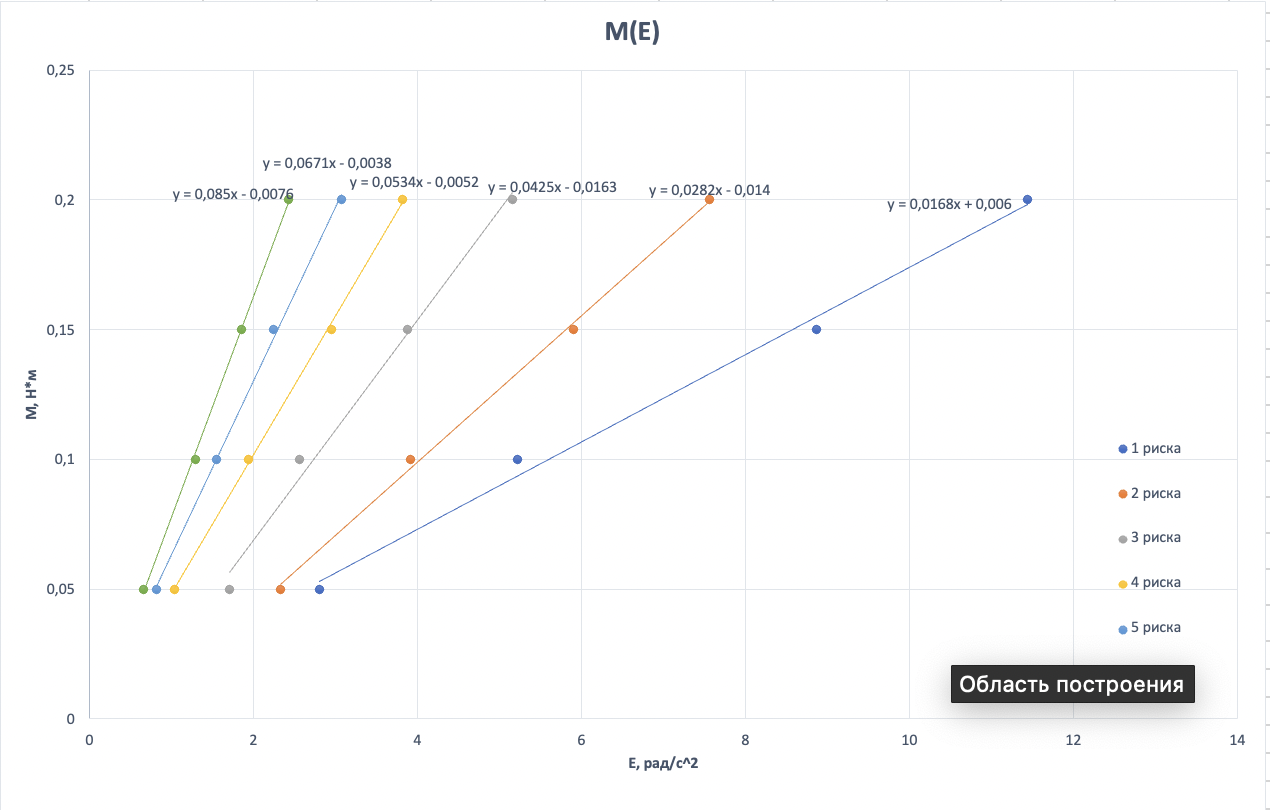
\includegraphics[width=1.05\linewidth]{1.png}
                \end{figure}
            \item График зависимости $I(R^2)$:
                \begin{figure}[H]
                    \centering
                    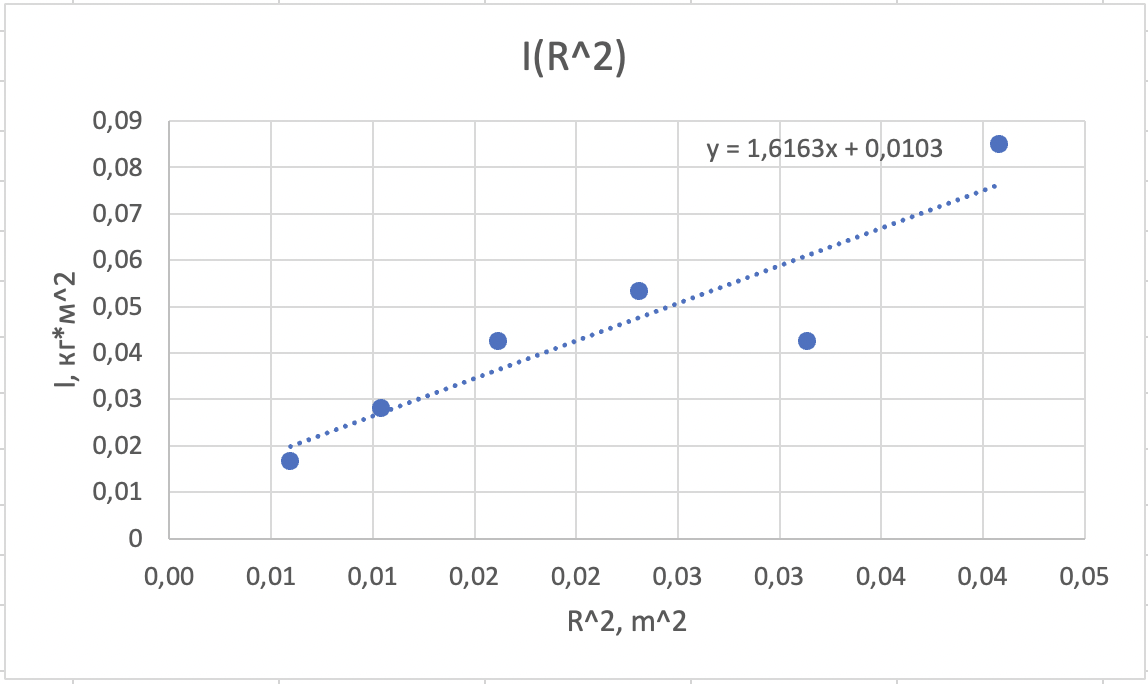
\includegraphics[width=1.05\linewidth]{2.png}
                    \label{fig:mpr}
                \end{figure}
        \end{itemize}
        
        \item Окончательные результаты.
        \begin{itemize} 
            \item Получены следующие величины:
            \begin{itemize}
                \item Первое значение $t_{\text{ср1}} = (4,66 \pm 0,21) c$
                \item Первое значение $a_{\text{ср1}} = (0,06 \pm 0,019) \frac{\text{м}}{c^2}$
                \item Первое значение $\varepsilon_{\text{ср1}} = (2,80 \pm 0,91) \frac{\text{рад}}{c^2}$
                \item Первое значение $M_{\text{ср1}} = (0,05 \pm 0,00..) \text{H*м}$
                \item Значение $m_{\text{ут}} = (0,61 \pm 0,001) H*\text{м}, \varepsilon = 1\%$
                \item Значение $I_0 = (0,01 \pm 0,003) \text{кг}*\text{м}^2, \varepsilon = 55\% $
                
                
        
            \end{itemize}
        
        
        \end{itemize}
        
        
        
        
        \item Выводы и анализ результатов работы.\\
        В ходе выполнения работы были получены зависимости $M(\varepsilon)$ и $I(R^2)$. Из графиков видно, что эта зависимость линейная, что подтверждает основной закон динамики вращения. 
        
        
    \end{enumerate}
    
\end{document}